% ADock technical report (4 pages). Build: bash scripts/build_technical_report.sh
% Tables weights_table.tex and gap_table.tex are written by scripts/make_summary_figures.py from config/ and predictions/.
\documentclass[10pt,a4paper,twocolumn]{article}
\usepackage[margin=1.5cm,top=1.4cm,bottom=1.6cm,columnsep=0.6cm]{geometry}
\usepackage{amsmath,amssymb}
\usepackage{graphicx}
\usepackage{booktabs}
\usepackage{tabularx}
\usepackage{enumitem}
\usepackage{xcolor}
\usepackage{titlesec}
\usepackage[font=small,labelfont=bf,skip=3pt]{caption}
\usepackage{algorithm}
\usepackage{algpseudocode}
\usepackage[hidelinks]{hyperref}
\usepackage{microtype}

\definecolor{accent}{HTML}{B34700}
\titleformat{\section}{\normalsize\bfseries\color{accent}}{\thesection}{0.6em}{}
\titleformat{\subsection}{\small\bfseries}{\thesubsection}{0.5em}{}
\titlespacing*{\section}{0pt}{6pt}{2pt}
\titlespacing*{\subsection}{0pt}{4pt}{1pt}
\setlist{itemsep=0.5pt,parsep=0pt,topsep=1.5pt,leftmargin=1.1em}
\setlength{\parskip}{2pt}
\setlength{\parindent}{0pt}
\setlength{\textfloatsep}{6pt}
\setlength{\floatsep}{5pt}
\setlength{\dbltextfloatsep}{6pt}
\newcommand{\file}[1]{\texttt{\footnotesize #1}}
\newcommand{\pp}{\,pp}

\begin{document}

\twocolumn[{
\begin{center}
{\Large\bfseries\color{accent} ADock: fast physics-based docking, and an AlphaFold gap\\[2pt] that physics cannot close\par}
\vspace{4pt}
{\small Technical report $\cdot$ October 2026 $\cdot$ produced by an AI-agent team (Claude Opus 5.5 / Sonnet 5.5) in 24\,h;\\
checked by independent agents, not yet reviewed by human experts. Full record: \file{docs/REPORT.md}.\par}
\end{center}
\vspace{2pt}
\begin{minipage}{\textwidth}\small
\textbf{Abstract.} We present ADock, a GPU reimplementation of AutoDock Vina-style docking with an 18-weight
interpretable scoring function, and use it to dissect why physics-based docking fails on AlphaFold (AF) receptors.
ADock docks a complex in 0.22\,s (Uni-Dock 2.7\,s, GNINA 10.2\,s) and reaches 58.6\,\% top-1 success on PoseBusters~V2,
level with Vina-family tools and GNINA without its neural network (59.3\,\%) but below GNINA with CNN rescoring
(67.0\,\%). On 222 complexes released after 2023, replacing the experimental receptor by its AF model lowers success
from 50.5 to 10.8\,\% (GNINA 61.3 to 16.7\,\%). On validation data, 13 attempted fixes---receptor softening,
side-chain repacking, rotamer and BioEmu2 ensembles, metal placement, AF-tolerant scoring, consensus, re-ranking,
force-field induced fit, homolog pocket transfer and co-folded receptors---do not close the gap. Oracle experiments
locate it in sub-\AA ngstr\"om geometry of backbone and side chains jointly: the true pocket recovers $+12$\pp, true
side chains alone do not help significantly. All three pre-registered confirmatory claims failed.
\end{minipage}
\vspace{8pt}
}]

\section{Introduction}

Structure-based docking predicts the bound pose of a small molecule in a protein pocket. Classical tools such as
AutoDock Vina~\cite{trott2010,eberhardt2021} combine a fast empirical score with stochastic search; GNINA~\cite{mcnutt2025}
adds a convolutional neural network (CNN) that rescores poses, and Uni-Dock~\cite{yu2023} moves Vina to the GPU. Two
needs motivate this work. First, proteome-scale docking needs sub-second cost per pocket. Second, most proteins have
no experimental structure, only an AlphaFold model~\cite{varadi2022}, and docking into AF models is known to lose much
of its accuracy~\cite{karelina2023,holcomb2023}. We built a fast engine (Sec.~\ref{sec:method}), benchmarked it under a
pre-registered protocol (Sec.~\ref{sec:holo}), and then asked what part of an AF pocket defeats physics-based scoring
(Sec.~\ref{sec:gap}).

\section{Setup}
\label{sec:setup}

\textbf{Task.} Pocket-given docking: the box is a fixed cube of edge $\max(24\,\text{\AA}, \text{extent}+4)$ centred on
the residues within 6\,\AA{} of the reference ligand, identical for every method. \textbf{Success} = top-1 pose within
2\,\AA{} symmetry-corrected heavy-atom RMSD of the crystal pose; timeouts (300\,s) count as failures.

\textbf{Receptors.} \emph{Holo}: the experimental structure solved with the ligand. \emph{AF}: the AlphaFold database
(AFDB) model of the same protein, superposed on the pocket C$\alpha$ atoms.

\textbf{Test sets} (locked and held out until one final run; seed 0 unless stated):
PoseBusters~V2~\cite{buttenschoen2024} (PB2, $n=285$, holo);
Runs N' Poses~\cite{skrinjar2025} $\cap$ PLINDER~\cite{durairaj2024} complexes released after 2023-06-01 ($n=222$; 178
with an AFDB v4 model), docked into both holo and AF receptors;
PB2 with AFDB and ESMFold receptors from PoseBench~\cite{morehead2025} ($n=268$); and a dimer-pocket set ($n=1080$).
The date cut keeps test complexes out of the AF and co-folding training data.

\textbf{Validation.} PLINDER, DockGen and Astex sets plus 125 post-2023 AF complexes, with no PDB, UniProt or PLINDER-cluster
overlap with the tests. Each set is split by UniProt into a \emph{selection} half (all choices) and a
\emph{confirmation} half (looked at once). The whole AF-gap diagnosis (Sec.~\ref{sec:gap}) uses validation data only.

\textbf{Comparators.} Vina~1.2, smina~\cite{koes2013}, Vinardo~\cite{quiroga2016}, Uni-Dock, GNINA~1.3 with and
without CNN rescoring. Claims, margins and tests were pre-registered (\file{config/preregistration.yaml}); a code guard
logged every test-data access.

\section{Method}
\label{sec:method}

\subsection{Scoring}
For a ligand pose $x$, the Vina inter-molecular energy sums over ligand--receptor atom pairs $(i,j)$ within 8\,\AA{}
terms of the surface distance $d_{ij} = r_{ij} - R_i - R_j$ ($R$: van der Waals radius of the X-Score atom type):
\begin{equation}
E_{\text{Vina}}(x) = \sum_{(i,j)} \sum_{k=1}^{5} w_k\, f_k(d_{ij}),
\end{equation}
with two Gaussian contact terms, a quadratic repulsion for $d<0$, and piecewise-linear hydrophobic and hydrogen-bond
terms. The \textbf{fitted score} keeps this form and adds eight features $\phi_k$ that are also functions of distance
and (extended) atom type only, so each still collapses into one precomputed grid per ligand atom type:
\begin{equation}
E_{\text{fit}}(x) = \sum_{k=1}^{13} w_k \Phi^{\text{inter}}_k(x) + \sum_{k=1}^{5} w'_k \Phi^{\text{intra}}_k(x).
\end{equation}
Receptor atoms are typed as buried when $\geq 177$ heavy atoms lie within 10\,\AA, and by formal charge (Lys, Arg, Asp,
Glu, C-terminus). With the new weights set to zero and the others to Vina's, $E_{\text{fit}}$ ranks poses exactly as Vina.

\textbf{Fit.} Poses come from fast ADock runs on 2,447 holo and 932 AF training complexes (released before
2021-10, disjoint from validation and test), plus the minimised crystal pose and perturbed copies; positives are
$\leq 2$\,\AA, decoys $>4$\,\AA, about 117,000 poses in total. The loss combines a softmax ranking term with
temperature $\tau$, a hinge term asking the minimised native pose to score below decoys, and an $L_2$ pull towards
Vina in feature-standard-deviation units (schematic; exact form in \file{src/adock/fit/}):
\begin{multline}
\mathcal{L}(w) = \sum_{c} \Big[ -\log \frac{\sum_{p \in P_c} e^{-E(p)/\tau}}{\sum_{x \in P_c \cup D_c} e^{-E(x)/\tau}}
 + \tfrac12\, h_c(w) \Big] \\ + \lambda \lVert s \odot (w - w_{\text{Vina}}) \rVert^2 ,
\end{multline}
optimised with L-BFGS ($\tau=1$, $\lambda=0.1$, chosen on a 10\,\% UniProt hold-out). Table~\ref{tab:weights} lists
the result. A shuffled-label control fitted on the same data scores below Vina (57 vs 66 of 336 validation successes).

\begin{table}[t]
\centering\footnotesize
\caption{Scoring weights (Vina default vs fitted; \file{config/adock\_fitted.json}). ``new'' terms are 0 in Vina.}
\label{tab:weights}
\begin{tabular}{@{}llrr@{}}
\toprule
group & term & Vina & fitted \\
\midrule
Vina & gauss1 (contact) & $-0.0356$ & $-0.0421$ \\
Vina & gauss2 (contact) & $-0.0052$ & $-0.0050$ \\
Vina & repulsion & $+0.8402$ & $+0.8157$ \\
Vina & hydrophobic & $-0.0351$ & $-0.0374$ \\
Vina & H-bond & $-0.5874$ & $-0.5993$ \\
new & buried hydrophobic & $+0.0000$ & $-0.0104$ \\
new & buried H-bond & $+0.0000$ & $-0.0334$ \\
new & ligand-donor H-bond & $+0.0000$ & $+0.0436$ \\
new & charged H-bond & $+0.0000$ & $-0.0590$ \\
new & metal--acceptor & $+0.0000$ & $-0.2891$ \\
new & ionic & $+0.0000$ & $+0.5160$ \\
new & polar--apolar & $+0.0000$ & $-0.0200$ \\
new & buried contact & $+0.0000$ & $-0.0096$ \\
intra & gauss1 & $-0.0356$ & $-0.0253$ \\
intra & gauss2 & $-0.0052$ & $-0.0046$ \\
intra & repulsion & $+0.8402$ & $+0.7775$ \\
intra & hydrophobic & $-0.0351$ & $-0.0231$ \\
intra & H-bond & $-0.5874$ & $-0.2060$ \\
\bottomrule
\end{tabular}

\end{table}

\begin{figure}[t]
\centering
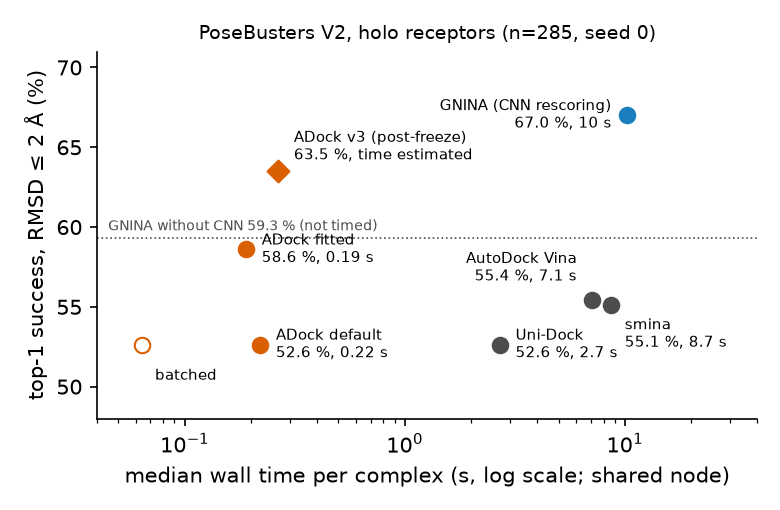
\includegraphics[width=\linewidth]{fig_speed_accuracy.png}
\caption{Speed vs accuracy on PB2 holo receptors ($n=285$, seed 0). Time: median per complex in one scripted
sequential pass over 50 complexes (6 cores each, shared node, so upper bounds). The v3 time is estimated
($1.4\times$ fitted, from validation).}
\label{fig:speed}
\end{figure}

\subsection{Search}
Algorithm~\ref{alg:search} follows Vina's Monte Carlo + BFGS scheme~\cite{trott2010,eberhardt2021}. Each search chain
runs in one GPU warp (32 threads share the energy and gradient evaluation of one pose), many chains and complexes run
per kernel launch (as in Uni-Dock~\cite{yu2023}), and grids are trilinearly interpolated on the GPU. Kernels are CUDA
compiled at run time (cupy NVRTC); the same source compiles with \texttt{g++ -fopenmp} for CPUs (energy agreement
$3\times10^{-6}$ relative; success within seed noise).

\begin{algorithm}[t]
\caption{ADock search for one complex}
\label{alg:search}
\footnotesize
\begin{algorithmic}[1]
\State build per-type grids of $E_{\text{fit}}$ over the box
\State Stage A: rigid-body enumeration to seed $N$ chains
\For{each chain $c = 1..N$ \textbf{in parallel} (one warp each)}
  \For{$s = 1..S$} \Comment{$S$ scales with ligand size}
    \State mutate one of position / orientation / torsion
    \State local BFGS on the grid energy
    \State accept with Metropolis criterion, $T=1.2$
  \EndFor
\EndFor
\State polish top chains on exact pairwise energy
\State rescore exactly, cluster, return ranked poses
\end{algorithmic}
\end{algorithm}

\textbf{Presets.} \texttt{v2\_default}: $N=256$ chains $\times$ 128 steps; \texttt{v2\_fitted}: same search with
$E_{\text{fit}}$; \texttt{v2\_fast}: 64 $\times$ 128; \texttt{v2\_accurate}: 512 $\times$ 256 with $4\times$ Stage A.
A post-freeze variant ``v3'' (fitted score, accurate search, repulsion capped at 1\,\AA$^2$) is exploratory.

\begin{figure*}[t]
\centering
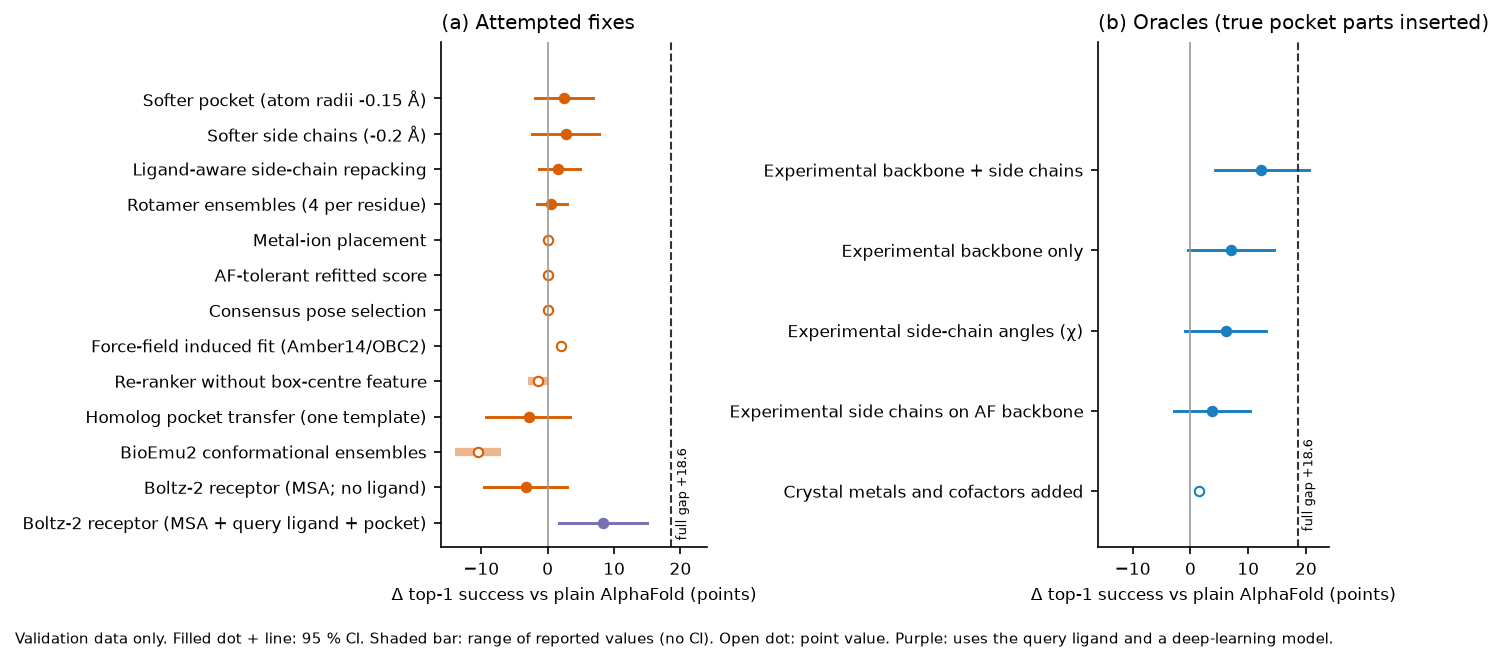
\includegraphics[width=0.94\textwidth]{fig_af_gap.png}
\caption{AF-gap diagnosis on validation data (post-2023 AF set, $n \approx 107$--125; 2--3 seeds). Change in top-1
success relative to ADock on the plain AF model. Dashed line: full holo$-$AF gap ($+18.6$\pp). (a) Attempted fixes.
(b) Oracles that replace parts of the AF pocket by the true (holo) coordinates. Values and sources per row:
\file{docs/summary/af\_gap\_arms.csv} (transcribed from \file{docs/REPORT.md} \S5, not recomputed).}
\label{fig:gap}
\end{figure*}

\section{Results on experimental receptors}
\label{sec:holo}


\textbf{Speed.} ADock takes 0.22\,s per complex warm (0.06\,s in batches), $12\times$ faster than Uni-Dock and
$46\times$ faster than GNINA (Fig.~\ref{fig:speed}). A 64-core node with one GPU (three GPU drivers plus the CPU engine)
processes 66 pockets/s, i.e.\ $\approx$4.2 node-hours per $10^6$ pockets (projection from benchmark pockets).

\textbf{Accuracy.} The fitted score raises ADock from 52.6 to 58.6\,\% on PB2, above Vina (55.4), smina (55.1) and
Uni-Dock (52.6; $+6.0$\pp, McNemar $p=0.017$), level with GNINA without CNN (59.3) and below GNINA with CNN (67.0) (Table~\ref{tab:holo}; example pose in Fig.~\ref{fig:pose}).
v3 adds $+4.9$\pp{} at seed 0 ($+3.5$ over three seeds; 63.5\,\%). In pockets formed by two different chains ADock
is non-inferior to GNINA (54.8 vs 43.5\,\%).

\begin{table}[t]
\centering\footnotesize
\caption{PB2 holo results ($n=285$). Top-1 success (\%) at seed 0 and over seeds 0--2 where all three were run;
median time per complex in the timing pass (``--'': not timed). Generated from \file{predictions/}.}
\label{tab:holo}
\begin{tabular}{@{}lrrr@{}}
\toprule
method & seed 0 & seeds 0--2 & time (s) \\
\midrule
ADock default & 52.6 & 53.6 $\pm$ 1.3 & 0.22 \\
ADock fitted & 58.6 & 60.2 $\pm$ 2.0 & 0.19 \\
Vina 1.2 & 55.4 & -- & 7.10 \\
smina & 55.1 & -- & 8.68 \\
Vinardo & 46.3 & -- & -- \\
Uni-Dock (balance) & 52.6 & 51.8 $\pm$ 0.9 & 2.70 \\
GNINA, no CNN & 59.3 & -- & -- \\
GNINA (CNN) & 67.0 & 69.0 $\pm$ 1.8 & 10.21 \\
\bottomrule
\end{tabular}

\end{table}

\begin{figure}[t]
\centering
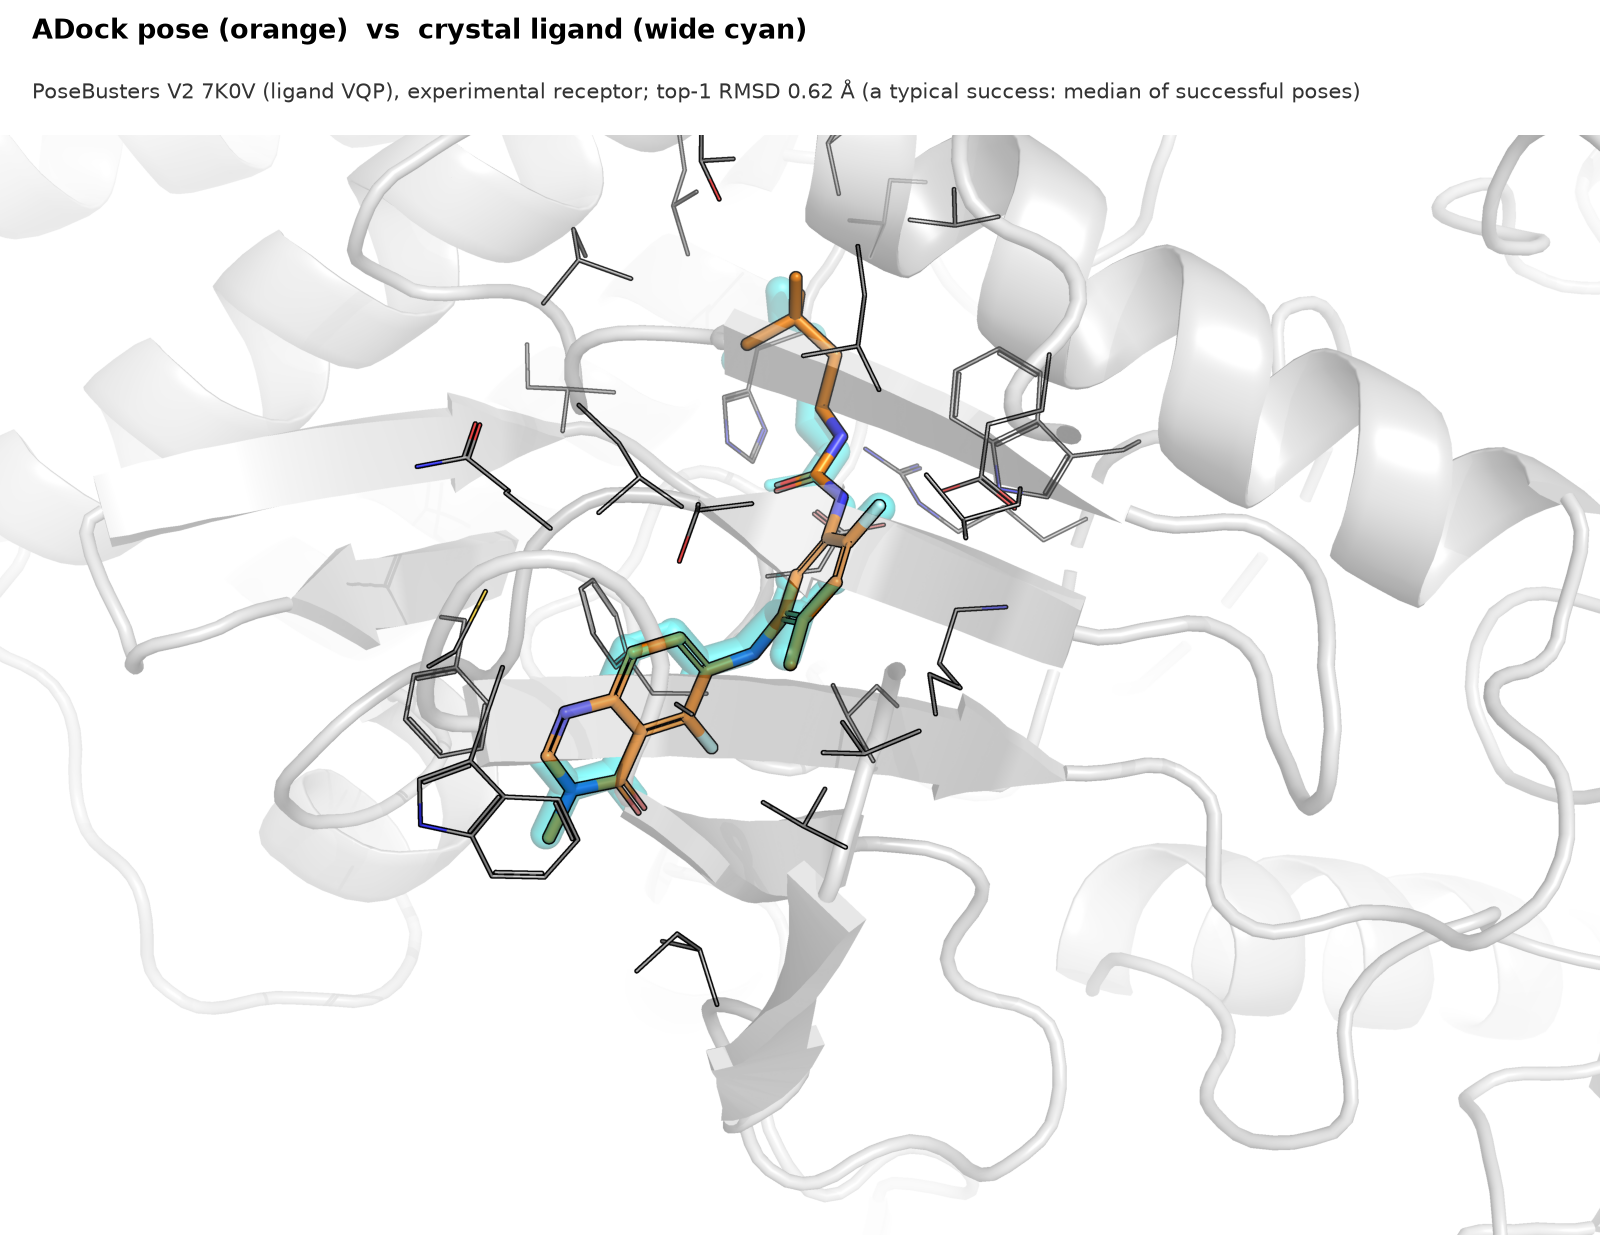
\includegraphics[width=\linewidth,trim=0 0 0 150,clip]{docked_example.png}
\caption{ADock pose (orange) and crystal ligand (wide cyan) for PDB 7K0V (PB2, holo receptor), top-1 RMSD 0.62\,\AA.
Chosen by a fixed rule: the median-RMSD success among ligands with 20--32 heavy atoms (v3 preset, seed 0;
\file{scripts/render\_docked\_example.py}).}
\label{fig:pose}
\end{figure}

\textbf{Pre-registered claims} (Holm over three): C1, ADock $\geq$ GNINA on AF receptors: 11.2 vs 18.0\,\%,
\emph{fail}. C2, faster and non-inferior (margin 3\pp) to GNINA and Uni-Dock: speed passes, accuracy fails (52.6 vs
67.0 / 52.6\,\%). C3, fitted ADock non-inferior (margin 5\pp) to the best physics comparator (GNINA without CNN):
58.6 vs 59.3\,\%, $p=0.042$, Holm-adjusted 0.13, \emph{not significant}.

\section{The AlphaFold gap}
\label{sec:gap}

\textbf{Size.} The same complexes lose 31--45 points when the holo receptor is replaced by its AF model, for ADock and
GNINA alike (Table~\ref{tab:gap}), although the AF pocket backbone lies a median 0.4--0.5\,\AA{} from holo.

\begin{table}[t]
\centering\footnotesize
\caption{Top-1 success (\%, seed 0) with experimental vs predicted receptors. RnP: Runs N' Poses post-2023 ($n=222$).
PB2: PoseBusters V2 with AFDB / ESMFold receptors ($n=268$).}
\label{tab:gap}
\resizebox{\columnwidth}{!}{\begin{tabular}{@{}lrrrrr@{}}
\toprule
 & RnP holo & RnP AF & $\Delta$ & PB2 AFDB & PB2 ESMF. \\
\midrule
ADock default & 42.8 & 12.2 & $-30.6$ & 7.5 & 8.6 \\
ADock fitted & 50.5 & 10.8 & $-39.6$ & 11.9 & 11.9 \\
GNINA (CNN) & 61.3 & 16.7 & $-44.6$ & 20.9 & 18.3 \\
\bottomrule
\end{tabular}
}
\end{table}


\textbf{Attempted fixes} (Fig.~\ref{fig:gap}a). \emph{Forgiving receptors}---radii softened by 0.15--0.2\,\AA,
ligand-aware rotamer repacking, rotamer ensembles, metal placement---gave $+0$ to $+3$\pp{}, all CIs including zero;
selection-half gains of $+7$ to $+9$ vanished on confirmation. \emph{Scoring and ranking}---a joint refit with
softness on AF receptors, consensus pose selection, a 16-feature conditional-logit re-ranker, and Amber14/OBC2
induced-fit refinement of the top poses with OpenMM---gave $-3$ to $+2$. \emph{Other receptors}: BioEmu2
ensembles~\cite{lewis2025} lost 7--14\pp{} (closest-of-24 pocket 1.48\,\AA{} from holo vs 0.89\,\AA{} for AF);
single-template homolog pocket transfer $-2.8$; Boltz-2~\cite{boltz} receptors co-folded with an MSA but without the
ligand $-3.3$. Only co-folding \emph{with the query ligand and a pocket constraint} helped ($+8.3$ [1.7, 15.0];
confirmation half $+6.0$, n.s.), closing less than half the gap with a deep-learning model and the ligand itself.

\textbf{Oracles} (Fig.~\ref{fig:gap}b). Holo side-chain angles on the AF backbone, holo side chains, or crystal metals
and cofactors recover 0--6\pp, none significant; the holo backbone alone $+7$ (n.s.); the full holo pocket
$+12.2$ [4.2, 20.6] (selection half $+22$). The gap therefore lies in the joint sub-\AA{} geometry of backbone and
side chains, contrary to the common view that rotamers are the main problem~\cite{holcomb2023}.

\textbf{Why physics fails.} Of AF failures, 53\,\% are scoring failures (the minimised crystal pose scores worse than
the top pose by a median 2.3\,kcal/mol, vs 0.4 in holo pockets), 39\,\% receptor failures (the crystal pose is not a
local minimum and drifts $>2$\,\AA) and 8\,\% search failures. A full force field ranks the crystal pose first by
interaction energy in only 25--40\,\% of AF pockets vs 42--52\,\% of holo pockets. A correct pose is among the top 20
in 35--41\,\% of AF cases, but no physical feature identified it.

\textbf{Caveats.} All of Sec.~\ref{sec:gap} except Table~\ref{tab:gap} is validation data with wide CIs; several arms
report ranges or point values; samples differ slightly between arms; oracle and pocket-transfer analyses were run
after the test evaluation (on validation data). An apparent $+8$ from the re-ranker came entirely from a box-centre
feature (the true ligand sits at the box centre by construction); a 3\,\AA{} box shift turned it into $-5$.

\textbf{Side note: pose transfer.} Copying the ligand pose from an earlier complex of a similar protein, as in
AlphaFill~\cite{hekkelman2023}, gave 23.6 vs 18.0\,\% for GNINA on AF test receptors ($p=0.077$, exploratory) but
11.8\,\% once templates with $\geq 30$\,\% identity were excluded. This reuses known complexes rather than fixing the
physics.

\section{Discussion}

\textbf{Insights.} (i) AF pockets are close but not close enough: sub-\AA{} errors of backbone and side chains together
cost physics docking most of its accuracy, and neither softening, rebuilding side chains, nor sampling recovers it.
(ii) The failure lies in the energy landscape, not in search; a full force field is misled about as much as Vina.
(iii) Generated conformations (BioEmu2, homolog pockets) were not closer to holo than AF itself. (iv) On holo
receptors, scoring---not search---limits classical docking; a small interpretable refit, driven mostly by metal and
desolvation terms, gives $+6$\pp.

\textbf{Research practice.} Selection-half gains of 6--9\pp{} shrank to 0--3\pp{} on confirmation in nearly every
arm; ceiling (oracle) experiments run first ruled out several planned arms; and every gain had to be checked against
how the benchmark was built.

\textbf{How the work evolved.} A design review by four reviewer agents fixed the post-2023 AF test and the shared box
rule (hour 1). Measuring the gap first on validation (GNINA 44 $\to$ 17\,\%, hour 5) made it the central question.
Engine parity with Vina at $\sim$40$\times$ lower time, with failures dominated by scoring, led to the fitted score
(hour 5); its selection-to-confirmation shrinkage ($+6$--8 $\to$ $+2.8$) set the evaluation rule (hour 6). The
side-chain oracle (hour 7) predicted the failure of the rotamer arms; the re-ranker artefact was caught before the
freeze; force-field, BioEmu2, pocket-transfer and co-folding arms and the full-pocket oracle followed (hours 8--20).

\textbf{Limitations.} The pocket is given (predicted pockets untested). Timings come from a shared node. Engine
changes after the fit moved validation results by a few complexes, and results depend slightly on batch composition.
For the highest accuracy on experimental structures GNINA's CNN remains about 8\pp{} better; on AF models of novel
proteins no tested method exceeds $\sim$20\,\%.

\textbf{Outlook.} The oracle bounds what a better pocket is worth ($+12$ to $+22$\pp{} on validation). Two routes
follow: pocket generators that predict holo-like backbone \emph{and} side chains to well below 1\,\AA{}, which
neither BioEmu2 nor homolog transfer achieved here; or scores that are robust to such errors, for example terms averaged
over pocket ensembles and learned with few parameters on paired AF/holo structures, or receptor uncertainty from
pLDDT/PAE. Both are untested. Any gain must also be checked with predicted pockets and shifted boxes.

\textbf{Reproducibility.} Methods were frozen at git tag \texttt{freeze-final} (code commit and config SHA-256
recorded in \file{config/final\_frozen.yaml}; the evaluation script refuses to run if they differ). Seeds 0--2 for
every stochastic method; confirmatory tests use seed 0. Statistics: exact McNemar tests for paired success,
paired bootstrap for non-inferiority bounds, Holm correction over C1--C3; an independent agent recomputed all claims
(differences $\leq 0.01$\pp) and 48 RMSDs with spyrmsd (max $|\Delta| = 0.0005$\,\AA). Deviations from the
pre-registration (amendments A1--A7) are listed in \file{docs/REPORT.md} \S7.

\textbf{Availability.} Code, configurations, pre-registration, test outcomes and per-complex statistics:
this repository (\file{README.md}; reproduction commands in \file{docs/REPORT.md} \S9).

\footnotesize\raggedright
\begin{thebibliography}{99}\setlength{\itemsep}{0pt}
\bibitem{trott2010} O.~Trott, A.~J.~Olson. AutoDock Vina. \emph{J. Comput. Chem.} 31:455, 2010. doi:10.1002/jcc.21334
\bibitem{eberhardt2021} J.~Eberhardt et al. AutoDock Vina 1.2.0. \emph{J. Chem. Inf. Model.} 2021. doi:10.1021/acs.jcim.1c00203
\bibitem{mcnutt2025} A.~T.~McNutt et al. GNINA 1.3. \emph{J. Cheminform.} 2025. doi:10.1186/s13321-025-00973-x
\bibitem{yu2023} Y.~Yu et al. Uni-Dock. \emph{J. Chem. Theory Comput.} 2023. doi:10.1021/acs.jctc.2c01145
\bibitem{varadi2022} M.~Varadi et al. AlphaFold Protein Structure Database. \emph{Nucleic Acids Res.} 50:D439, 2022. doi:10.1093/nar/gkab1061
\bibitem{karelina2023} M.~Karelina, J.~J.~Noh, R.~O.~Dror. How accurately can one predict drug binding modes using AlphaFold models? \emph{eLife} 2023. doi:10.7554/eLife.89386
\bibitem{holcomb2023} M.~Holcomb et al. Evaluation of AlphaFold2 structures as docking targets. \emph{Protein Sci.} 2023.
\bibitem{buttenschoen2024} M.~Buttenschoen, G.~M.~Morris, C.~M.~Deane. PoseBusters. \emph{Chem. Sci.} 2024. doi:10.1039/D3SC04185A
\bibitem{skrinjar2025} P.~\v{S}krinjar et al. Have protein--ligand co-folding methods moved beyond memorisation? bioRxiv 2025. doi:10.1101/2025.02.03.636309
\bibitem{durairaj2024} J.~Durairaj et al. PLINDER. bioRxiv 2024. doi:10.1101/2024.07.17.603955
\bibitem{morehead2025} A.~Morehead et al. PoseBench. \emph{Nat. Mach. Intell.} 2025. arXiv:2405.14108
\bibitem{koes2013} D.~R.~Koes, M.~P.~Baumgartner, C.~J.~Camacho. smina. \emph{J. Chem. Inf. Model.} 2013. doi:10.1021/ci300604z
\bibitem{quiroga2016} R.~Quiroga, M.~A.~Villarreal. Vinardo. \emph{PLoS ONE} 2016. doi:10.1371/journal.pone.0155183
\bibitem{lewis2025} S.~Lewis et al. BioEmu. \emph{Science} 2025. doi:10.1101/2024.12.05.626885
\bibitem{boltz} J.~Wohlwend et al. Boltz-1 / Boltz-2. https://github.com/jwohlwend/boltz; doi:10.1101/2024.11.19.624167
\bibitem{hekkelman2023} M.~L.~Hekkelman et al. AlphaFill. \emph{Nat. Methods} 20:205, 2023. doi:10.1038/s41592-022-01685-y
\end{thebibliography}

\end{document}
